%!TEX root = ../hycas2010.tex
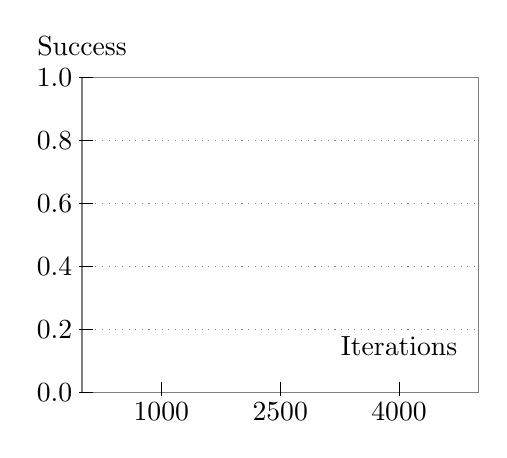
\begin{tikzpicture}[x=0.001cm,y=4cm]
    % Draw the axes and grid lines
    \draw[-,gray] (0,0) -- (0,1) -- (5000,1) -- (5000,0) -- cycle; 
    \draw[-,gray,thin, dotted, ystep=0.2, xstep=5000] (0,0) grid (5000,1);
    \foreach \x in {1000, 2500, 4000}  \draw [-,xshift=0](\x,4pt) -- (\x,-1pt);
    \foreach \y in {0.0,0.2,0.4,0.6,0.8,1.0}  \draw [-,yshift=0](4pt,\y) -- (-1pt,\y);
    \foreach \x/\xtext in {1000/1000, 2500/2500, 4000/4000} \node at (\x,0) [below] {$\xtext$};
    \foreach \y/\ytext in {0.0,0.2,0.4,0.6,0.8,1.0}  \node at (0,\y) [left] {$\ytext$};
    \node at (0,1.1) {Success};
    \node at (4000,0.15) {Iterations};
    \draw[-,gray] plot[mark=+,mark size=4,mark options={color=black}] 
			file {data/hanoid5s1r8.CF.tikzdata};
    \draw[-,gray] plot[mark=o,mark size=3,mark options={color=black}] 
			file {data/hanoid5s3r8.CF.tikzdata};
    \draw[-,gray] plot[mark=x,mark size=4,mark options={color=black}] 
			file {data/hanoid5s5r8.CF.tikzdata};

\end{tikzpicture}
